%%%%%%%%%%%%%%%%%%%%%%%%%%%%%%%%% LHS results %%%%%%%%%%%%%%%%%%
\begin{frame}{Echantillonnage par Latin Hypercube Sampling (LHS)}
    \begin{block}{}
        Objectif : Explorer l'espace et proposer une borne inférieure
        
    \end{block}\vspace*{-10pt}
    \begin{columns}
        %%%%%%%%%%%%%%%%%%%%%%%%%% COLONNE DE GAUCHE %%%%%%%%%%%%%%
        \begin{column}{0.35\textwidth} 

            \begin{figure}
                \centering
                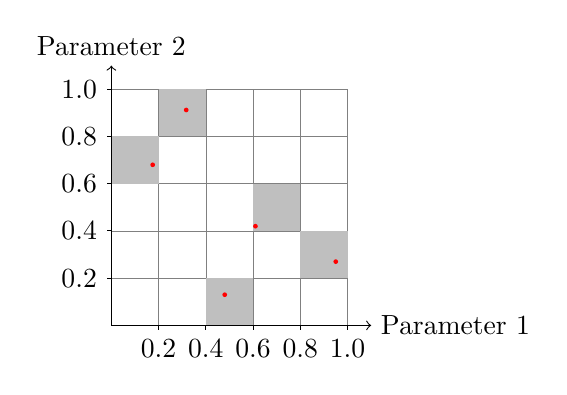
\begin{tikzpicture}[scale=3]

    % Define the grid
    \draw[step=0.2,gray,very thin] (0,0) grid (1,1);
    
    % Shade specific squares
    \fill[gray!50] (0.0,0.6) rectangle (0.2,0.8);
    \fill[gray!50] (0.2,0.8) rectangle (0.4,1.0);
    \fill[gray!50] (0.4,0.0) rectangle (0.6,0.2);
    \fill[gray!50] (0.6,0.4) rectangle (0.8,0.6);
    \fill[gray!50] (0.8,0.2) rectangle (1.0,0.4);
    
    % Draw red points
    \fill[red] (0.175,0.68) circle (0.01);  % Point in the first square
    \fill[red] (0.317,0.912) circle (0.01);  % Point in the second square
    \fill[red] (0.48,0.13) circle (0.01);  % Point in the third square
    \fill[red] (0.61,0.42) circle (0.01);  % Point in the fourth square
    \fill[red] (0.95,0.27) circle (0.01);  % Point in the fifth square
    
    % Draw the axes
    \draw[->] (0,0) -- (1.1,0) node[right] {Parameter 1};
    \draw[->] (0,0) -- (0,1.1) node[above] {Parameter 2};
    
    % Add ticks and labels
    \foreach \x in {0.2,0.4,0.6,0.8,1.0} {
      \draw (\x,0) -- (\x,-0.02) node[below] {\x};
      \draw (0,\x) -- (-0.02,\x) node[left] {\x};
    }
    
\end{tikzpicture}
                \caption{Illustration du Latin Hypercube Sampling avec $g=5$}
            \end{figure} 
     
            \end{column}
                 
         %%%%%%%%%%%%%%%%%%%%%%%%% COLONNE DE DROITE %%%%%%%%%%%%%%
            \begin{column}{0.55\textwidth}
                \begin{figure}
                    \centering
                    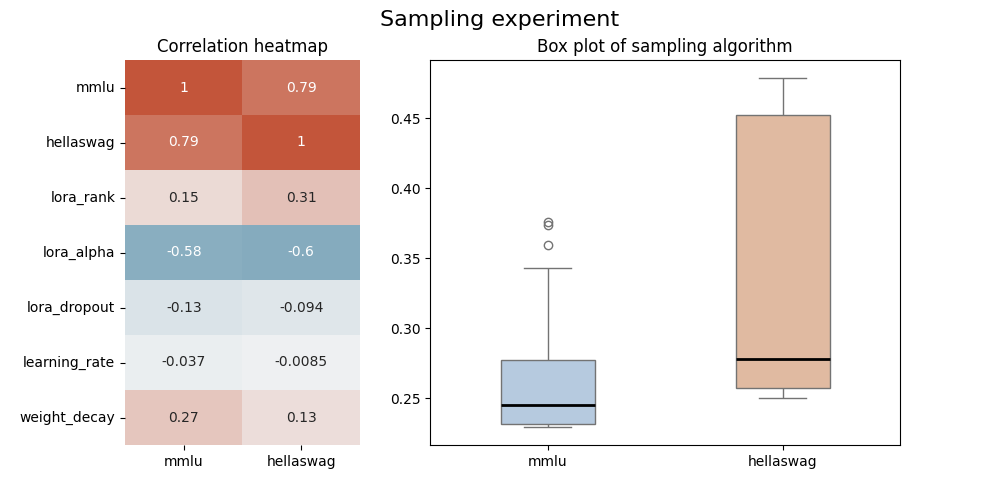
\includegraphics[width = \textwidth]{assets/imgs/plots/sampling/lhs.png}
                    \vspace*{-20pt}\caption{Résumé des résultats par sampling}
                \end{figure} 
            \end{column}
                 
    \end{columns}
\end{frame}

%%%%%%%%%%%%%%%%%%%%%%%%%%%%%%%%% Résultats %%%%%%%%%%%%%%%%%%
\begin{frame}{Résultats des 3 algorithms}
    \begin{columns}
        \begin{column}{0.45\textwidth}
            \begin{figure}
                \centering
                \begin{tikzpicture}[domain = 0:50,scale = 0.7]
    \tikzstyle{point} = [only marks, mark = triangle*, mark size = 3, opacity = 0.5]
    \begin{axis}[
        legend pos=south east,
        ymin = 0.2,
        x=3.2,
        y =700
    ]
    \addplot [blue,point, visible on = <1> ] table {assets/tikz_picture/global_results/bo_mmlu.dat};
    \addlegendentry{BO}

    \addplot [red, point, visible on = <2>] table {assets/tikz_picture/global_results/soo_mmlu.dat};
    \addlegendentry{SOO}

    \addplot [violet, point, visible on = <3>] table {assets/tikz_picture/global_results/bamsoo_mmlu.dat};
    \addlegendentry{BaMSOO}



    \addplot [blue,point, visible on = <4>] table {assets/tikz_picture/global_results/bo_mmlu.dat};
    \addplot [red, point, visible on = <4>] table {assets/tikz_picture/global_results/soo_mmlu.dat};
    \addplot [violet, point, visible on = <4>] table {assets/tikz_picture/global_results/bamsoo_mmlu.dat};




    \end{axis}
\end{tikzpicture}
                \caption{Résultats sur MMLU (test)}
            \end{figure}
        \end{column}
        \begin{column}{0.45\textwidth}
            \begin{figure}
                \centering
                \begin{tikzpicture}[domain = 0:50,scale = 0.7]
    \tikzstyle{point} = [only marks, mark = triangle*, mark size = 3, opacity = 0.5]
    \begin{axis}[
        legend pos=south east,
        ymin = 0.2,
        x=3.2,
        y =450
    ]
    \addplot [blue,point, visible on = <1>] table {assets/tikz_picture/global_results/bo_hellaswag.dat};
    \addlegendentry{BO}

    \addplot [violet, point, visible on = <2>] table {assets/tikz_picture/global_results/bamsoo_hellaswag.dat};
    \addlegendentry{BaMSOO}

    \addplot [red, point, visible on = <3>] table {assets/tikz_picture/global_results/soo_hellaswag.dat};
    \addlegendentry{SOO}

    \addplot [blue,point, visible on = <4>] table {assets/tikz_picture/global_results/bo_hellaswag.dat};
    \addplot [violet, point, visible on = <4>] table {assets/tikz_picture/global_results/bamsoo_hellaswag.dat};
    \addplot [red, point, visible on = <4>] table {assets/tikz_picture/global_results/soo_hellaswag.dat};



    \end{axis}
\end{tikzpicture}
                \caption{Résultats sur Hellaswag (Validation)}
            \end{figure}
        \end{column}
    \end{columns}
\end{frame}

%%%%%%%%%%%%%%%%%%%%%%%%%%%%%%%%% Analyse %%%%%%%%%%%%%%%%%%
\begin{frame}{Analyse}
    \begin{table}[h!]
        \centering
        \begin{tabular}{|c||c|c||c|c|c|}
        \hline
           Jeu de données  & Borne Inf.$^1$& Borne Sup.$^2$ & BO-GP & SOO & BaMSOO \\
        \hline
           Hellaswag (validation)  & 47.90 & \textit{41.5} & \textbf{47.91} & 47.84 & 47.84\\
           MMLU (testing) & 37.61 & 49.3 & \textbf{38.11} & 37.42 & 37.50 \\
        \hline
        \end{tabular}
        \caption{Bornes et meilleurs résultats sur les 2 jeu de données}
    \end{table}
    \vspace*{-5pt}{\footnotesize 1 : expérience avec LHS; 2 : Fine tuning par Meta}

    \begin{block}{Points clés}     
    \end{block}
    
    \vspace*{-15pt}
    \begin{columns}
        
        %%%%%%%%%%%%%%%%%%%%%%%%%% COLONNE DE GAUCHE %%%%%%%%%%%%%%
        \begin{column}{0.45\textwidth} 
                \begin{itemize}
                    \item Borne Sup. sur Hellaswag non pertinente
                    \item Seul BO arrive au dessus de LHS
                    \item BaMSOO n'améliore que peu SOO
                \end{itemize}
        \end{column}  
         %%%%%%%%%%%%%%%%%%%%%%%%% COLONNE DE DROITE %%%%%%%%%%%%%%
            \begin{column}{0.45\textwidth}
                \begin{itemize}
                    \item principe de BaMSOO fonctionnel (visible annexe \ref{ap:bamsoo_results})
                    \item Espace de solution n'évolue que peu, le retravailler pour mesurer pleinement la performance des algorithmes
                \end{itemize}
            \end{column}          
    \end{columns}
    
\end{frame}

%%%%%%%%%%%%%%%%%%%%%%%%%%%%%%%%% Perspectives %%%%%%%%%%%%%%%%%%

\begin{frame}{Perspectives}
    \begin{columns}
        
        %%%%%%%%%%%%%%%%%%%%%%%%%% COLONNE DE GAUCHE %%%%%%%%%%%%%%
        \begin{column}[t]{0.45\textwidth} 
            \begin{block}{Poursuite du travail}
                \begin{itemize}
                    \item Retour sur l'article et présentation en conférence (si validation)
                    \item Elargissement de l'espace de recherche
                    \item Diversification sur les modèles/données
                \end{itemize}                
            \end{block}

        \end{column}  
         %%%%%%%%%%%%%%%%%%%%%%%%% COLONNE DE DROITE %%%%%%%%%%%%%%
            \begin{column}[t]{0.45\textwidth}
                \begin{block}{Optimisation fractale parallèle enrichie par approche bayésienne\footnote[3]{\textit Parallel Bayesian-enhanced Fractals Optimization}}

                    \begin{itemize}
                        \item Généralisation de l'hybridation décomposition/bayésien dans un cadre parallèle
                        \begin{itemize}
                            \item 5 moyens d'exploiter le \textit{surrogate} pour améliorer l'optimisation fractale
                        \end{itemize}
                    \end{itemize}
                \end{block}
            \end{column}
        
                 
    \end{columns}
    
\end{frame}